% Options for packages loaded elsewhere
\PassOptionsToPackage{unicode}{hyperref}
\PassOptionsToPackage{hyphens}{url}
\documentclass[
  ignorenonframetext,
]{beamer}
\newif\ifbibliography
\usepackage{pgfpages}
\setbeamertemplate{caption}[numbered]
\setbeamertemplate{caption label separator}{: }
\setbeamercolor{caption name}{fg=normal text.fg}
\beamertemplatenavigationsymbolsempty
% remove section numbering
\setbeamertemplate{part page}{
  \centering
  \begin{beamercolorbox}[sep=16pt,center]{part title}
    \usebeamerfont{part title}\insertpart\par
  \end{beamercolorbox}
}
\setbeamertemplate{section page}{
  \centering
  \begin{beamercolorbox}[sep=12pt,center]{section title}
    \usebeamerfont{section title}\insertsection\par
  \end{beamercolorbox}
}
\setbeamertemplate{subsection page}{
  \centering
  \begin{beamercolorbox}[sep=8pt,center]{subsection title}
    \usebeamerfont{subsection title}\insertsubsection\par
  \end{beamercolorbox}
}
% Prevent slide breaks in the middle of a paragraph
\widowpenalties 1 10000
\raggedbottom
\AtBeginPart{
  \frame{\partpage}
}
\AtBeginSection{
  \ifbibliography
  \else
    \frame{\sectionpage}
  \fi
}
\AtBeginSubsection{
  \frame{\subsectionpage}
}
\usepackage{iftex}
\ifPDFTeX
  \usepackage[T1]{fontenc}
  \usepackage[utf8]{inputenc}
  \usepackage{textcomp} % provide euro and other symbols
\else % if luatex or xetex
  \usepackage{unicode-math} % this also loads fontspec
  \defaultfontfeatures{Scale=MatchLowercase}
  \defaultfontfeatures[\rmfamily]{Ligatures=TeX,Scale=1}
\fi
\usepackage{lmodern}
\ifPDFTeX\else
  % xetex/luatex font selection
\fi
% Use upquote if available, for straight quotes in verbatim environments
\IfFileExists{upquote.sty}{\usepackage{upquote}}{}
\IfFileExists{microtype.sty}{% use microtype if available
  \usepackage[]{microtype}
  \UseMicrotypeSet[protrusion]{basicmath} % disable protrusion for tt fonts
}{}
\makeatletter
\@ifundefined{KOMAClassName}{% if non-KOMA class
  \IfFileExists{parskip.sty}{%
    \usepackage{parskip}
  }{% else
    \setlength{\parindent}{0pt}
    \setlength{\parskip}{6pt plus 2pt minus 1pt}}
}{% if KOMA class
  \KOMAoptions{parskip=half}}
\makeatother
\usepackage{longtable,booktabs,array}
\usepackage{caption}
\captionsetup[table]{skip=6pt}
\newcounter{none} % for unnumbered tables
\usepackage{calc} % for calculating minipage widths
\usepackage{caption}
% Make caption package work with longtable
\makeatletter
\def\fnum@table{\tablename~\thetable}
\makeatother
\usepackage{graphicx}
\makeatletter
\newsavebox\pandoc@box
\newcommand*\pandocbounded[1]{% scales image to fit in text height/width
  \sbox\pandoc@box{#1}%
  \Gscale@div\@tempa{\textheight}{\dimexpr\ht\pandoc@box+\dp\pandoc@box\relax}%
  \Gscale@div\@tempb{\linewidth}{\wd\pandoc@box}%
  \ifdim\@tempb\p@<\@tempa\p@\let\@tempa\@tempb\fi% select the smaller of both
  \ifdim\@tempa\p@<\p@\scalebox{\@tempa}{\usebox\pandoc@box}%
  \else\usebox{\pandoc@box}%
  \fi%
}
% Set default figure placement to htbp
\def\fps@figure{htbp}
\makeatother
\setlength{\emergencystretch}{3em} % prevent overfull lines
\providecommand{\tightlist}{%
  \setlength{\itemsep}{0pt}\setlength{\parskip}{0pt}}
% Auto-generated by infrastructure/rendering/_pdf_latex_helpers.py::extract_math_font_preamble.
% Minimal header passed to Pandoc via -H so Beamer slides pick up the same math font
% as the combined-PDF path. Adjust the manuscript's preamble.md to change the font globally.
\usepackage{unicode-math}
\setmathfont{latinmodern-math.otf}

% Manuscript macro/package fallbacks (newcommand -> providecommand).
% Core mathematics
\usepackage{amsmath}
\usepackage{amssymb}
% Document layout
% Tables
\usepackage{booktabs}
% Algorithm typesetting (for pseudocode in §2 Methodology)
% Code listings
\usepackage{listings}
% Typography and formatting
% Cross-references and citations
% ── Unicode-capable mono font for code listings ──────────────────────
% JuliaMono (TeX Live 2026) covers the full math/Greek glyph set used in
% scientific code blocks; the default lmmono lacks \alpha/\mu/\partial/\nabla.
%
% The hardcoded TeX Live 2026 path below is portable to most macOS / Linux
% TeX Live installs that placed JuliaMono under the default texmf-dist path.
% If your TeX Live version differs (e.g., 2025, 2027) or your distribution
% installs fonts elsewhere, comment out the explicit Path = line — fontspec
% will then search the system font path. If JuliaMono is not installed at
% all, comment out the whole block; xelatex falls back to lmmono with
% reduced Unicode coverage but the document still compiles.
% Math font for unicode-math: Latin Modern Math (TeX Live) has full BMP
% coverage including U+2223 (\mid), U+226A/226B (\ll/\gg), and the Greek/
% blackboard letters used in equations. Without an explicit \setmathfont,
% unicode-math falls back to lmroman text font which lacks several glyphs
% and emits "Missing character" warnings on every \mid in math mode.

% Slide layout defaults for warning-clean scientific decks.
\usepackage{etoolbox}
\IfFileExists{xurl.sty}{\usepackage{xurl}}{}
\IfFileExists{seqsplit.sty}{\usepackage{seqsplit}}{\newcommand{\seqsplit}[1]{#1}}
\protected\def\breakseq#1{\seqsplit{#1}}
\protected\def\breaktt#1{\begingroup\ttfamily\seqsplit{#1}\endgroup}
\setlength{\emergencystretch}{6em}
\tolerance=5000
\hbadness=10000
\hfuzz=1pt
\setlength{\tabcolsep}{2pt}
\AtBeginEnvironment{longtable}{\tiny\renewcommand{\arraystretch}{0.86}\setlength{\tabcolsep}{1pt}}
\AtBeginEnvironment{tabular}{\tiny\renewcommand{\arraystretch}{0.86}\setlength{\tabcolsep}{1pt}}
\AtBeginEnvironment{equation}{\tiny}
\AtBeginEnvironment{equation*}{\tiny}
\AtBeginEnvironment{align}{\tiny}
\AtBeginEnvironment{align*}{\tiny}
\AtBeginEnvironment{itemize}{\footnotesize}
\AtBeginEnvironment{enumerate}{\footnotesize}
\AtBeginEnvironment{description}{\footnotesize}
\setbeamerfont{caption}{size=\tiny}
\setbeamerfont{caption name}{size=\tiny}
\setbeamerfont{normal text}{size=\small}
\setbeamerfont{frametitle}{size=\small}
\setbeamerfont{section title}{size=\footnotesize}
\setbeamerfont{subsection title}{size=\footnotesize}
\setbeamertemplate{section page}{%
  \centering
  \begin{beamercolorbox}[sep=12pt,center,wd=\paperwidth]{section title}
    \parbox{0.86\paperwidth}{\centering\usebeamerfont{section title}\insertsection\par}
  \end{beamercolorbox}
}
\setbeamertemplate{subsection page}{%
  \centering
  \begin{beamercolorbox}[sep=8pt,center,wd=\paperwidth]{subsection title}
    \parbox{0.86\paperwidth}{\centering\usebeamerfont{subsection title}\insertsubsection\par}
  \end{beamercolorbox}
}
\setlength{\abovecaptionskip}{2pt}
\setlength{\belowcaptionskip}{0pt}

% Natbib and cross-reference fallbacks — slides don't load natbib
% or cleveref, but combined-PDF manuscript prose may emit these
% commands. The fallback renders citations as a bracketed key list
% and cross-references as detokenized labels so slides don't fail on
% undefined control sequences or raw underscores. \providecommand is
% a no-op if packages load later.
\providecommand{\citep}[1]{[#1]}
\providecommand{\citet}[1]{#1}
\providecommand{\citealp}[1]{#1}
\providecommand{\citeauthor}[1]{#1}
\providecommand{\citeyear}[1]{#1}
\providecommand{\cref}[1]{\texttt{\detokenize{#1}}}
\providecommand{\Cref}[1]{\texttt{\detokenize{#1}}}
\providecommand{\crefrange}[2]{\texttt{\detokenize{#1}}--\texttt{\detokenize{#2}}}
\providecommand{\Crefrange}[2]{\texttt{\detokenize{#1}}--\texttt{\detokenize{#2}}}
\providecommand{\paragraph}[1]{\textbf{#1}\ }

\newtheorem{proposition}{Proposition}
\newtheorem{hypothesis}{Hypothesis}
\newtheorem{remark}[theorem]{Remark}
\newtheorem{axiom}{Axiom}
\newtheorem{property}{Property}
\usepackage{bookmark}
\IfFileExists{xurl.sty}{\usepackage{xurl}}{} % add URL line breaks if available
\urlstyle{same}
% fallback for those not using the hyperref driver hyperxmp:
\makeatletter
\@ifundefined{xmpquote}{\newcommand{\xmpquote}[1]{#1}}{}
\makeatother
\hypersetup{
  hidelinks,
  pdfcreator={LaTeX via pandoc}}

\author{\texorpdfstring{}{}}
\date{}

\begin{document}

\section{Forecast: 2028--2031}\label{sec:forecast}

\begin{frame}[allowframebreaks]{Forecast: 2028--2031}
The forecasts in this section cover the 2028--2031 horizon. They are
reasoned expectations drawn from documented designs, the capability
evidence assembled in sec.~3, and the platform
reviews of sec.~5 through sec.~9. They
are not commitments, not measurements, and not claims about any
project's roadmap or release schedule. Official assessments bracket the
near end of the horizon, and both are recent enough to describe the
posture the forecast extends. The UK NCSC's assessment published in May
2025 at CYBERUK --- its second look after the January 2024 original
(Centre 2024) --- projects AI-assisted reconnaissance, vulnerability
research, exploit development, and social engineering through a 2027
horizon, while considering fully automated, end-to-end advanced attacks
unlikely within it (Centre 2026). A year later, the CISA-led Five Eyes
guidance on careful adoption of agentic AI services states the defensive
\end{frame}

\begin{frame}[allowframebreaks]{Forecast: 2028--2031}
counterpart: sandboxed deployment, early agents restricted to low-risk
tasks, threat-model-based evaluation, and red-teaming as adoption
prerequisites (Cybersecurity and Agency 2026). Together the two
documents are the current official posture: offense is accelerating
inside known boundaries, and defenders are advised to adopt capability
under containment rather than withhold it. DARPA's AIxCC results anchor
the defensive engineering side within the same bracket:
machine-discovered and machine-patched vulnerabilities, including real
non-synthetic flaws, are already demonstrated (DARPA 2025). The forecast
assumes both curves move through and beyond the bracket. It declines to
assume that attacker capability improves while defensive engineering
stands still.
\end{frame}

\begin{frame}[allowframebreaks]{Highest-confidence architectural bets}
\protect\phantomsection\label{highest-confidence-architectural-bets}
The forecast register records 14 claims: 5 high-confidence architectural
bets, 4 execution-dependent outcomes, and 5 claims the analysis declines
to endorse. The high-confidence bets are architectural in a specific
sense: each follows from the structure of the threat rather than from
any vendor's plans.

\textbf{Compartmentalization value grows with exploitation frequency.}
If offensive automation raises how often exposed components fail,
architectures that protect the rest of the system after a failure gain
value mechanically. This supports Qubes-like strict domain separation
and disposable execution --- not as a claim that any hypervisor is
unbreakable, but because QSB-118's route from an already-compromised
qube to dom0 command injection under specified conditions shows both the
value of the boundaries and the standing obligation to patch the
\end{frame}

\begin{frame}[allowframebreaks]{Highest-confidence architectural bets}
management plane that guards them (Q. O. Project 2026c).

\textbf{Capability mediation becomes as important as exploit
mitigation.} More capable agents raise the value of distinguishing what
an agent can propose from what it can authorize
(sec.~10). Operating-system isolation and
application-level, API-level authorization must work together; neither
substitutes for the other, which is the property independence of
sec.~4 applied forward.

\textbf{Fast, trustworthy replacement beats elaborate repair.} Against
uncertain compromise, rebuilding from known-good configuration plus
credential revocation dominates forensic repair on an unverified footing
--- especially when authorized misuse may have left no exploit trace at
all (sec.~12). This favors declarative and image-based
operations, with mutable data and secrets handled separately rather than
swept into the rebuild (sec.~6).

\end{frame}

\begin{frame}[allowframebreaks]{Highest-confidence architectural bets}
\textbf{Small interfaces deserve disproportionate investment.} The
components that move bytes, credentials, approvals, and device access
across domains are natural targets. Their size, privilege,
implementation language, and policy semantics can matter more than the
number of isolated workloads on the other side of them. qrexec's
policy-mediated request channel (Q. O. Project 2026a) and the
GUI/admin-domain disaggregation in Qubes 4.3 (Q. O. Project 2026b) are
instances of the pattern: concentrate care where authority crosses.

\end{frame}

\begin{frame}[allowframebreaks]{Highest-confidence architectural bets}
\textbf{Coherent defaults beat optional hardening menus.} A baseline
that survives browser updates, developer workflows, and ordinary
maintenance is worth more than many switches operators cannot safely
combine. The maintainer discussion proposing deprecation of NixOS's
hardened profile documents the failure mode directly: a menu of
restrictions without a coherent baseline can undermine browser
sandboxing unless compensating setup is supplied ({community} 2026b).
\end{frame}

\begin{frame}[allowframebreaks]{Execution-dependent trajectories}
\protect\phantomsection\label{execution-dependent-trajectories}
Three trajectories are promising but decided by execution rather than
architecture.

\textbf{Qubes: disaggregation without fragility.} Qubes 4.3 moves
complex components --- the GUI stack, administrative services --- out of
the most privileged domain, alongside new device-assignment mechanisms
and initial Wayland work (Q. O. Project 2026b). The open question is
whether the resulting reduction in privileged attack surface arrives
without operational fragility that pushes users to collapse their
compartments, which would trade the human-usability property for the
containment property. The trajectory is the right one; its delivery
conditions are not yet settled.

\end{frame}

\begin{frame}[allowframebreaks]{Execution-dependent trajectories}
\textbf{NixOS: confinement and integrity as one baseline.} The open
question is whether reproducible configuration integrates with a
coherent confinement and integrity baseline --- the security wiki
documents incomplete SELinux and AppArmor integration, and Lanzaboote
remains in development ({community} 2026c, 2026a) --- rather than
remaining largely an operator-assembled composition. The composable
potential is real (sec.~6); whether it becomes a
maintained default rather than a skilled operator's assembly job is an
execution question. The support lifecycle sharpens it: NixOS 26.05's
seven-month window of security fixes, ending December 31, 2026, makes an
explicit update process a precondition of any claim on the platform (N.
Project 2026).

\end{frame}

\begin{frame}[allowframebreaks]{Execution-dependent trajectories}
\textbf{Conventional desktops: permission narrowing while usable.}
secureblue documents allocator hardening, a confined browser, removal of
SUID-root programs, and deliberate namespace restrictions (secureblue
Project 2026); Flatpak's own documentation describes a restrictive base
sandbox whose permission grants expand access and warns about
unrestricted bus access (F. Project 2026). The trajectory question is
whether application permissions and agent authority narrow substantially
while remaining usable --- whether the desktop permission model
converges on something operators keep rather than disable.
\end{frame}

\begin{frame}[allowframebreaks]{The attractive destination}
\protect\phantomsection\label{the-attractive-destination}
The composition worth building toward is a compartmentalized system
whose small privileged services are memory-safe where feasible, whose
core security properties carry strong verification (Klein et al. 2009),
whose boot and update paths authenticate the intended software, and
whose environments can be independently rebuilt. Each property closes a
different failure class: containment for exploitation, verification for
defects in privileged services, authenticated update for supply-chain
substitution, rebuildability for persistence and unauthorized change.
None substitutes for the others --- that non-substitutability is the
property independence of sec.~4 restated as
a design program. The destination is a composition, and composition
quality is precisely what no reviewed product yet supplies as a default
(sec.~5; sec.~6; sec.~7).
fig.~\ref{fig:forecast_horizon} arranges the registered forecasts by
\end{frame}

\begin{frame}[allowframebreaks]{The attractive destination}
confidence tier across the horizon.

\end{frame}

\begin{frame}[allowframebreaks]{The attractive destination}
\begin{figure}
\centering
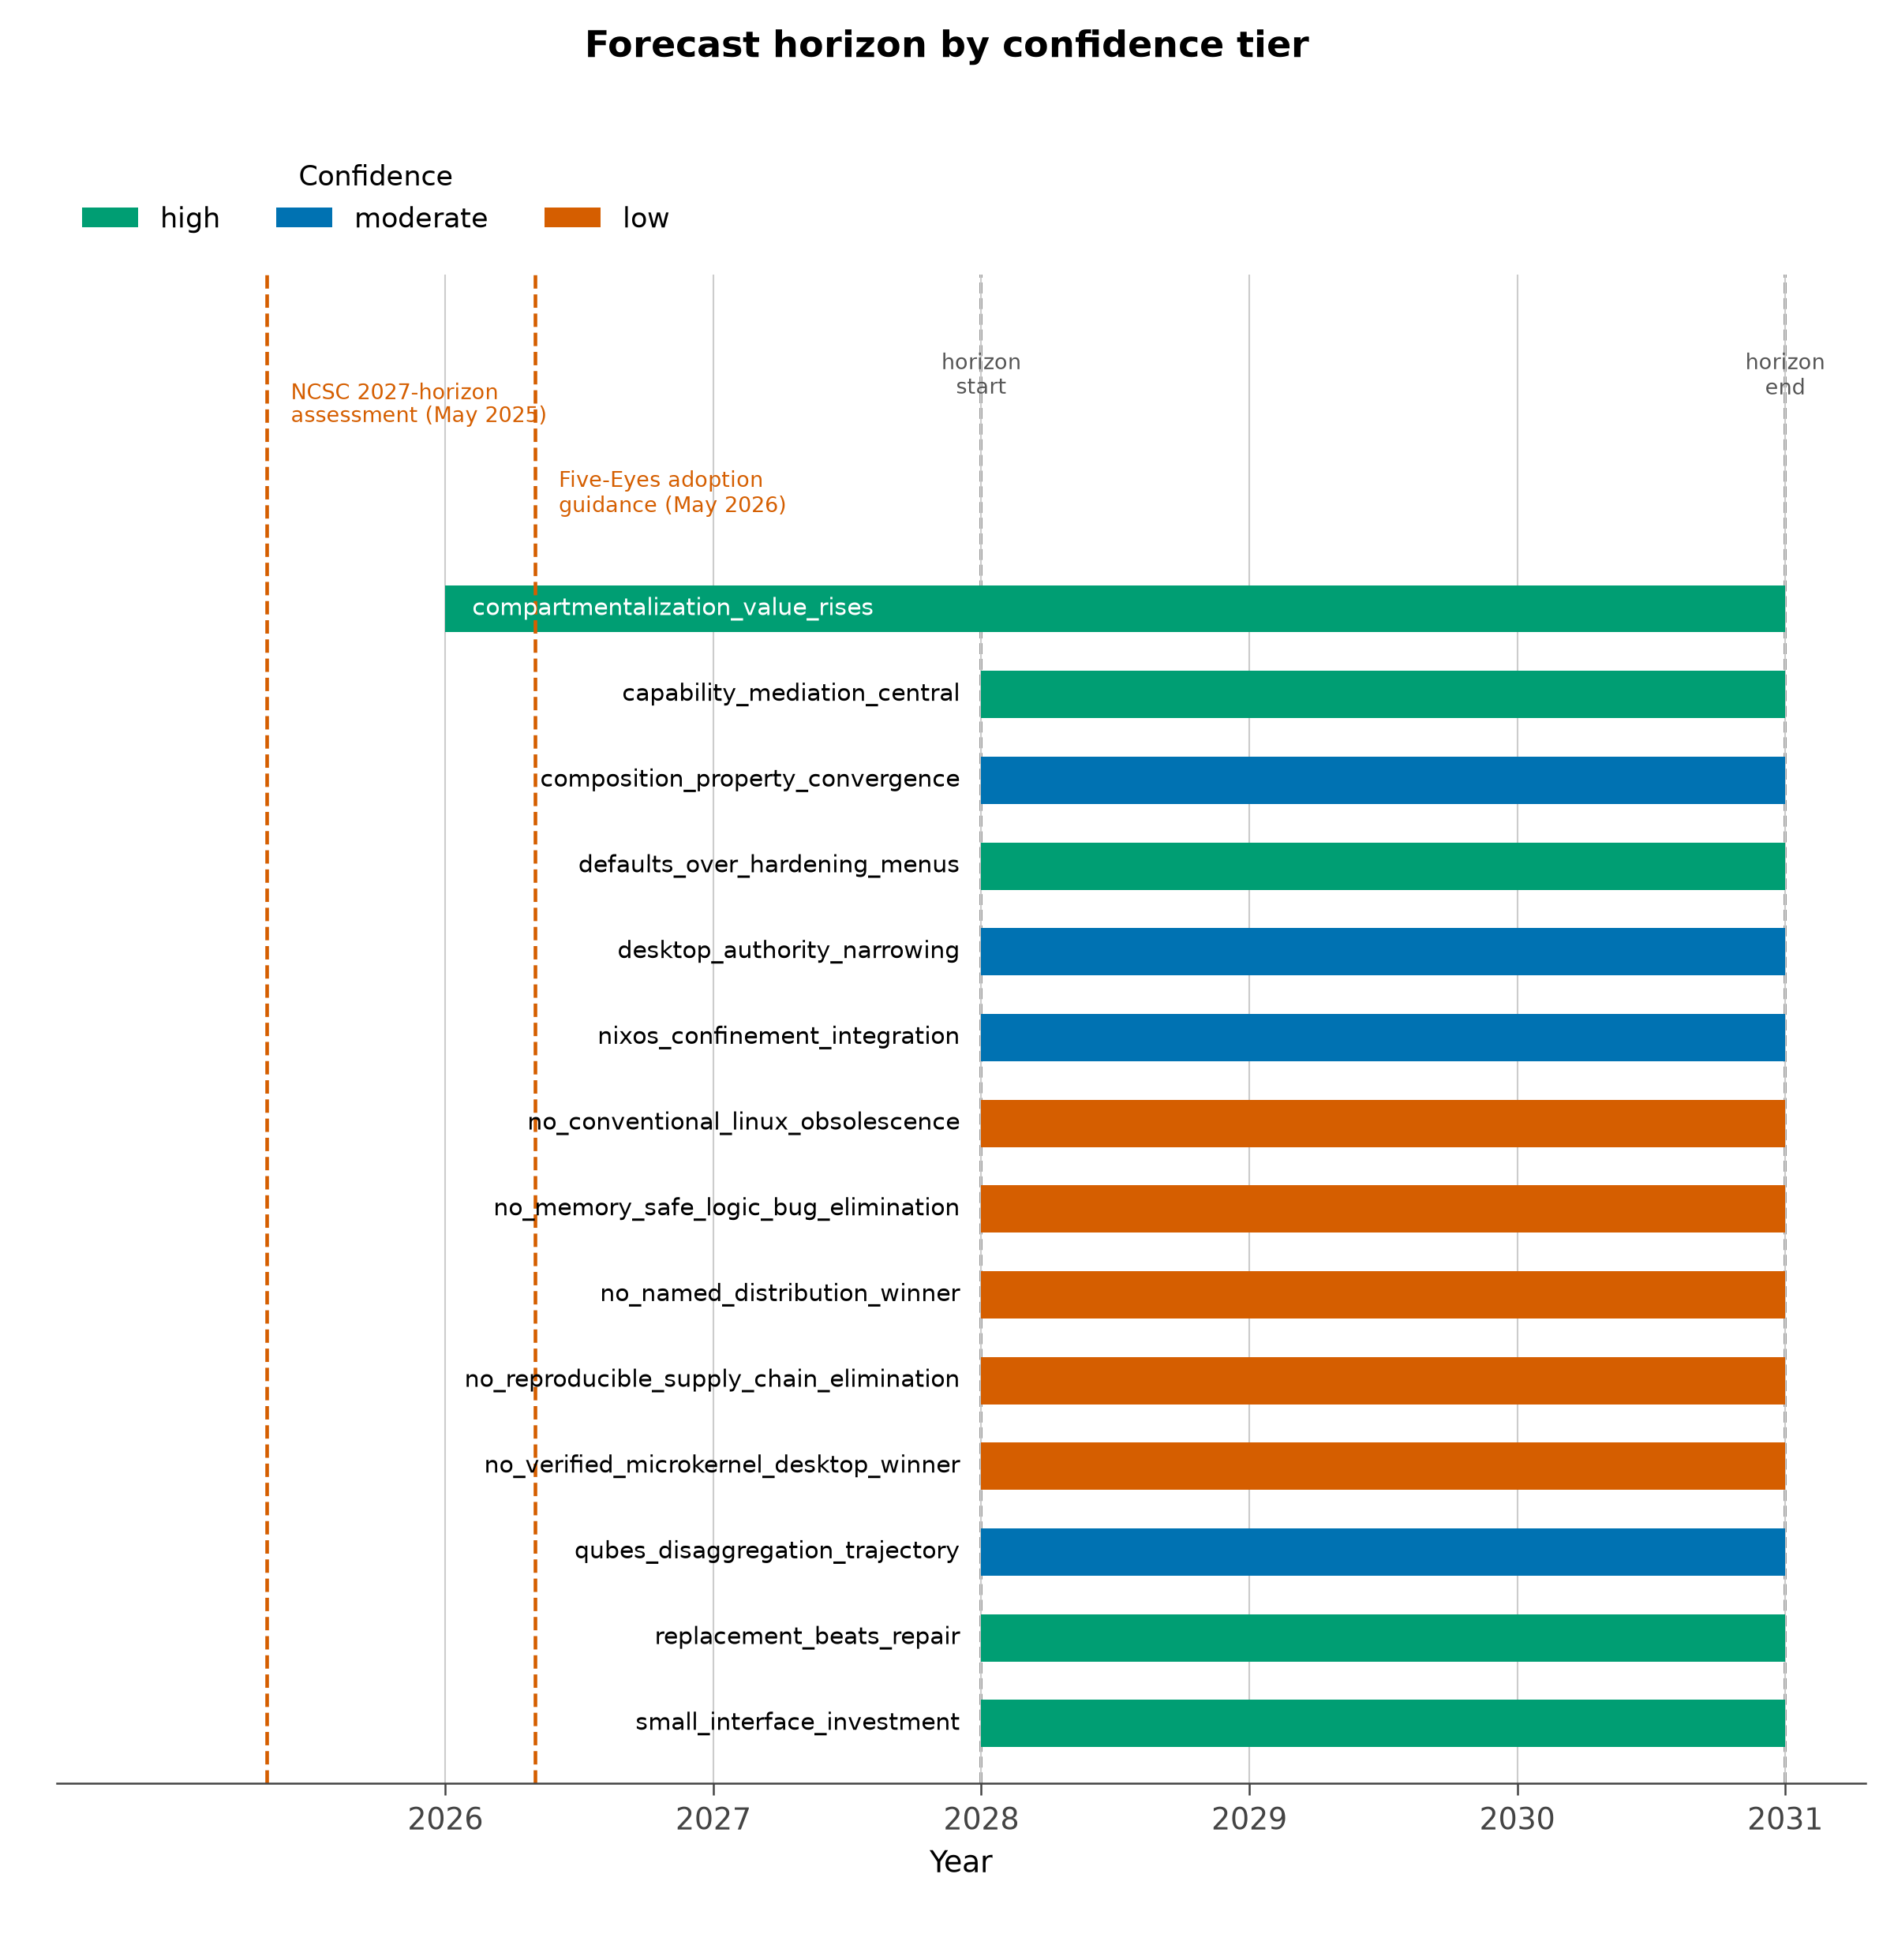
\includegraphics[width=1\linewidth,height=0.40\textheight,keepaspectratio,alt={The 2028--2031 forecast horizon: the registered forecast claims grouped by confidence tier --- high-confidence architectural bets, moderate execution-dependent outcomes, and low-confidence claims the analysis declines to endorse --- across operating-system architecture, agent authority, and supply-chain domains. The horizon bounds this review's expectations; it is not a release schedule for any project.}]{../figures/forecast_horizon.png}
\caption{The 2028--2031 forecast horizon: the registered forecast claims
grouped by confidence tier --- high-confidence architectural bets,
moderate execution-dependent outcomes, and low-confidence claims the
analysis declines to endorse --- across operating-system architecture,
agent authority, and supply-chain domains. The horizon bounds this
review's expectations; it is not a release schedule for any
project.}\label{fig:forecast_horizon}
\end{figure}
\end{frame}

\begin{frame}[allowframebreaks]{Forecasts this analysis declines}
\protect\phantomsection\label{forecasts-this-analysis-declines}
Four forecasts would be overconfident, and naming them is part of the
forecast. A verified microkernel does not automatically yield the best
practical desktop: seL4's proofs are scoped to the kernel under stated
hardware and boot assumptions (Foundation 2026; Klein et al. 2009), and
a verified core does not verify the browser, the driver stack, the
firmware chain, or the workflow. A memory-safe rewrite does not
eliminate logic vulnerabilities: memory safety removes one defect class
while confused-deputy and authorization defects remain fully available
(Hardy 1988). Reproducible packages do not eliminate supply-chain
compromise: reproducibility plus signature verification establish build
integrity, not source benignity, and a trusted signer can still
distribute a harmful artifact ({community} 2026d). And conventional
Linux is not obsolete merely because offensive agents improve:
\end{frame}

\begin{frame}[allowframebreaks]{Forecasts this analysis declines}
maintenance quality, deployment competence, and reachable authority
decide outcomes, and a competently maintained conventional system can
outrun an ambitiously isolated but neglected one. Each declined forecast
fails the same way --- it substitutes one property for the whole
composition.
\end{frame}

\begin{frame}[allowframebreaks]{The decisive uncertainty}
\protect\phantomsection\label{the-decisive-uncertainty}
The main uncertainty is not whether additional isolation can be useful.
It is which projects can deliver stronger boundaries, usable delegation,
reliable updates, and sufficient compatibility together, without pushing
users into insecure workarounds. Under offensive-AI pressure, the
operative failure mode shifts from missing protection to abandoned
protection: the compartment the operator collapses under deadline
pressure, the update process that decays, the delegation that widens for
convenience (sec.~11). A forecast about
architecture is therefore always partly a forecast about maintenance and
ergonomics. The 2028--2031 window will be decided less by any single
breakthrough than by which compositions people can actually keep.
\end{frame}

\end{document}
